\documentclass[conference]{IEEEtran}

\usepackage{cite}
\usepackage{amsmath,amssymb,amsfonts}
\usepackage{algorithmic}
\usepackage{graphicx}
\usepackage{textcomp}
\usepackage{xcolor}
\usepackage{booktabs}
\usepackage{array}
\usepackage{multirow}
\usepackage{url}
\usepackage{tikz}
\usetikzlibrary{arrows.meta,positioning,fit,shapes.geometric,calc}

\def\BibTeX{{\rm B\kern-.05em{\sc i\kern-.025em b}\kern-.08em
    T\kern-.1667em\lower.7ex\hbox{E}\kern-.125emX}}

\begin{document}

\title{Explainable AI-Driven Risk Scoring for Fraud Analyst Decision Support}

\author{
\IEEEauthorblockN{1\textsuperscript{st} Agjelia Lydia C.}
\IEEEauthorblockA{\textit{Department of Information Technology} \\
\textit{Karpagam College of Engineering} \\
Coimbatore 641032, Tamil Nadu, India}
\and
\IEEEauthorblockN{2\textsuperscript{nd} Kanis Krishna K A}
\IEEEauthorblockA{\textit{Department of Information Technology} \\
\textit{Karpagam College of Engineering} \\
Coimbatore 641032, Tamil Nadu, India}
\and
\IEEEauthorblockN{3\textsuperscript{rd} Mukesh M.}
\IEEEauthorblockA{\textit{Department of Information Technology} \\
\textit{Karpagam College of Engineering} \\
Coimbatore 641032, Tamil Nadu, India}
\and
\IEEEauthorblockN{4\textsuperscript{th} Santhosh A S}
\IEEEauthorblockA{\textit{Department of Information Technology} \\
\textit{Karpagam College of Engineering} \\
Coimbatore 641032, Tamil Nadu, India}
\and
\IEEEauthorblockN{5\textsuperscript{th} Barath R.}
\IEEEauthorblockA{\textit{Department of Information Technology} \\
\textit{Karpagam College of Engineering} \\
Coimbatore 641032, Tamil Nadu, India}
}

\maketitle

\begin{abstract}
Financial fraud detection systems in operational transaction monitoring units confront two acute operational bottlenecks: overwhelming alert queues dominated by false positives and opaque machine learning risk estimates that fail to disclose the behavioural drivers governing an alert. This paper presents an explainable, human-in-the-loop decision-support platform engineered to assist fraud analysts in triaging, investigating, and adjudicating suspicious financial transactions. The proposed architecture decouples an offline Python-based machine learning pipeline from a MongoDB-backed Java Spring Boot REST API and a React analyst dashboard. Customer spending baselines are synthesized dynamically from historical transaction streams, capturing deviations across transaction amount, velocity, frequency, circadian timing, device transitions, and geographic displacement across 38 engineered features. An XGBoost classifier estimates posterior fraud probabilities, while TreeSHAP produces exact local feature attributions and global feature rankings in margin space. Evaluated on an out-of-time chronological partition of 550 transactions (40 fraudulent, 510 legitimate) derived from a schema-compliant IEEE-CIS benchmark dataset, the proposed model achieves 92.31\% precision, 90.00\% recall, a ROC-AUC of 0.9975, and a PR-AUC of 0.9668, yielding only three false positives. A paired non-parametric bootstrap analysis over 1,000 resamples confirms that incorporating behavioural and velocity features yields a statistically significant PR-AUC improvement of 0.0279 over the transaction-only baseline (bootstrap mean difference: 0.0269, 95\% CI: [0.0035, 0.0589], $p = 0.0090$). Benchmark measurements confirm sub-85\,ms mean API response latencies, with four automated temporal leakage checks and 19 functional integration tests passing. The system is designed strictly for decision support, empowering analyst adjudication without autonomous transaction blocking.
\end{abstract}

\begin{IEEEkeywords}
fraud detection, explainable AI, XGBoost, SHAP, behavioural profiling, risk scoring, decision support, class imbalance, temporal leakage prevention, batch processing
\end{IEEEkeywords}

\section{Introduction}

Financial fraud in electronic payment gateways, banking networks, and digital commerce platforms causes tens of billions of dollars in economic damage annually~\cite{sarna2026ai}. While supervised machine learning models, including gradient-boosted trees and deep neural architectures, have become standard for automated transaction scoring, their practical efficacy in operational fraud investigation units and security operations centres (SOCs) is frequently impaired by operational alert fatigue and model opacity~\cite{lipton2016mythos,chan2015using}. A high volume of false-positive alerts exhausts human review capacity, while an uninterpretable probability score fails to provide actionable context for analysts who must determine whether to contact cardholders, freeze credit facilities, or dismiss alerts.

A fundamental difficulty in fraud surveillance arises from the substantial variance in individual consumer behaviour~\cite{bolton2002unsupervised}. A transaction of \$1,000 may represent routine spending for a corporate account but constitute an acute anomaly for a student. Uniform, population-wide threshold rules invariably produce elevated false-alarm rates for affluent cardholders while failing to intercept low-value account takeover (ATO) attacks or automated micro-structuring fraud~\cite{fetaji2025ai}.

While individualized behavioural profiling can capture these deviations, constructing dynamic customer baselines introduces an acute risk of \textit{temporal data leakage}~\cite{jurgovsky2018sequence}. If transactions from future intervals or out-of-time labels inadvertently contaminate historical rolling statistics, reported model accuracy becomes artificially inflated and degrades upon deployment. Furthermore, fraud datasets exhibit extreme class imbalance, where legitimate transactions outnumber fraudulent events by orders of magnitude~\cite{damanik2025advanced,zheng2025integrated}. Under these conditions, standard evaluation metrics such as overall accuracy and ROC-AUC can mask poor performance on the minority class; Precision-Recall AUC (PR-AUC) and absolute false-positive counts provide far more operationally meaningful assessments.

To address these challenges, this study presents FinGuard, an explainable AI-driven decision-support platform that combines causal customer behavioural profiling, tree-boosted risk scoring, and TreeSHAP feature attributions within a decoupled batch architecture. The primary contributions of this work are:
\begin{enumerate}
    \item \textbf{Causal Behavioural Feature Engineering:} Formulation of a 38-feature catalog capturing customer-specific amount deviations, circadian timing patterns, rolling velocity spikes, and spatial displacements. All aggregations enforce a strict causal lookback constraint ($t_j < t_i$), validated through automated temporal leakage tests.
    \item \textbf{Statistically Grounded Feature Ablation:} A paired non-parametric bootstrap analysis over 1,000 resamples on a chronologically held-out test partition demonstrating that adding behavioural and velocity features achieves a statistically significant PR-AUC lift of 0.0279 ($p = 0.0090$, 95\% CI: [0.0035, 0.0589]) over transaction-only attributes.
    \item \textbf{Operationally Aligned Model Selection:} An empirical evaluation comparing XGBoost, Random Forest, and Logistic Regression on identical chronological test data. While Random Forest achieves higher recall (97.50\% vs.\ 90.00\%), XGBoost achieves the highest precision (92.31\%) and the lowest false-positive count (3 vs.\ 4 for RF, 8 for LR), reducing analyst alert fatigue while providing native TreeSHAP compatibility.
    \item \textbf{Probability Calibration Analysis:} Evaluation of raw versus post-hoc calibrated probabilities (Platt scaling and isotonic regression), demonstrating that well-regularized gradient-boosted trees with positive-class weighting yield well-calibrated posterior probabilities directly (ECE: 0.0116, Brier score: 0.0108).
    \item \textbf{Decoupled Four-Tier Architecture:} Implementation of an asynchronous system separating offline Python batch processing from a Java Spring Boot REST API (sub-85\,ms mean latency) and a React dashboard that presents risk-ranked queues alongside additive SHAP waterfall attributions.
    \item \textbf{Human-Centered Triage Workflow:} A triage interface designed to support analyst adjudication through auditable status transitions and investigator notes, ensuring that automated scores guide but never replace human judgement.
\end{enumerate}

The remainder of this paper is organized as follows. Section~II surveys related work. Section~III formulates the problem and research objectives. Section~IV details the proposed system architecture. Section~V outlines the dataset and preprocessing pipeline. Section~VI formalizes behavioural feature engineering. Section~VII presents the fraud risk scoring methodology. Section~VIII describes explainable AI using SHAP. Section~IX provides experimental results and ablation studies. Section~X describes system implementation and performance. Section~XI discusses findings and limitations. Section~XII concludes the paper.

\section{Related Work}

Research on automated financial fraud detection encompasses rule-based filtering, unsupervised profiling, supervised machine learning, deep learning architectures, and explainable AI (XAI). Table~\ref{tab:related_work} compares these dominant paradigms.

\begin{table*}[t]
\centering
\caption{Comparison of Fraud Detection Approaches}
\label{tab:related_work}
\small
\begin{tabular}{lllll}
\toprule
\textbf{Approach} & \textbf{Representative Literature} & \textbf{Key Strengths} & \textbf{Primary Operational Limitations} \\
\midrule
Rule-Based Filtering & Bolton \& Hand~\cite{bolton2002unsupervised} & Deterministic, auditable, low latency & High false positives, rigid thresholds, manual maintenance \\
Unsupervised Profiling & Bolton \& Hand~\cite{bolton2002unsupervised} & Detects emerging anomalies without labels & Cannot distinguish fraud from benign shifts, high noise \\
Supervised Linear Classifiers & Chan et al.~\cite{chan2015using}, AlSagri~\cite{alsagri2025hybrid} & Fast training, interpretable coefficients & Inability to capture non-linear feature interactions \\
Tree Ensembles (RF, XGBoost) & Breiman~\cite{breiman2001random}, Chen \& Guestrin~\cite{chen2016xgboost} & High discriminative power, tabular efficiency & Opaque internal logic without post-hoc explainers \\
Class-Imbalance Handlers & Chawla et al.~\cite{chawla2002smote}, Damanik \& Liu~\cite{damanik2025advanced} & Improves minority recall on skewed sets & Synthetic samples risk distorting true temporal distributions \\
Cost-Sensitive Learning & Ileberi \& Sun~\cite{ileberi2025performance} & Aligns loss penalties with financial exposure & Requires exact cost matrices often unavailable in practice \\
Temporal \& Drift Adapters & Al Lawati et al.~\cite{allawati2025integrated}, Zheng et al.~\cite{zheng2025integrated} & Adapts to evolving fraud patterns & Complex online architectures, latency overhead \\
Graph Neural Networks & Offon~\cite{offon2026hybrid}, Sarwosri et al.~\cite{sarwosri2026ecommerce} & Captures syndicate rings and account links & High compute cost, privacy constraints across entities \\
Explainable AI (TreeSHAP) & Lundberg \& Lee~\cite{lundberg2017unified}, Lundberg et al.~\cite{lundberg2020local} & Exact additive game-theoretic attributions & Post-hoc explanations do not guarantee real-world causality \\
\textbf{Proposed FinGuard} & \textbf{This Study} & \textbf{Causal profiling, TreeSHAP, low false alarms} & \textbf{Asynchronous batch scoring; requires analyst review} \\
\bottomrule
\end{tabular}
\end{table*}

\subsection{Supervised Classification and Class Imbalance}
Supervised learning algorithms have largely superseded static rules in transaction monitoring~\cite{sarna2026ai,bolton2002unsupervised}. Early deployments utilized linear models and Logistic Regression for their interpretability; however, linear decision boundaries fail to model complex non-linear feature interactions~\cite{alsagri2025hybrid}. Random Forests~\cite{breiman2001random} and Gradient Boosted Decision Trees (XGBoost)~\cite{chen2016xgboost} have emerged as strong performers on tabular data, capturing intricate dependencies with high computational efficiency.

Extreme class imbalance remains an intrinsic property of transactional data, where fraud prevalence typically ranges between 0.1\% and 7\%~\cite{jurgovsky2018sequence}. Common responses to imbalance include synthetic oversampling such as SMOTE~\cite{chawla2002smote} and K-SMOTEENN~\cite{damanik2025advanced}, cost-sensitive oversampling~\cite{ileberi2025performance}, and temporal generative adversarial networks (TD-GAN)~\cite{zheng2025integrated}. In gradient boosting implementations, the positive-class loss weight parameter (\texttt{scale\_pos\_weight}) can be adjusted directly to penalize false negatives without generating synthetic instances that distort real-world transaction distributions~\cite{chen2016xgboost,han2025enhanced}.

\subsection{Behaviour-Based Fraud Indicators}
Static transaction attributes (such as transaction amount and merchant category) are frequently insufficient to detect account takeover (ATO) attacks where unauthorized actors transact within common amount ranges. Behavioural profiling mitigates this vulnerability by tracking individual spending baselines over rolling temporal horizons~\cite{allawati2025integrated}. Metrics such as amount-to-mean ratios, historical standard deviation Z-scores, inter-transaction velocity gaps, and device transition counters enable models to distinguish genuine cardholder behaviour from compromise. The IEEE-CIS Fraud Detection benchmark~\cite{ieee2019fraud} provides a standard tabular framework for evaluating these identity and behavioural interactions.

\subsection{Explainability for Fraud Decision Support}
Regulatory frameworks, including the European Union General Data Protection Regulation (GDPR) and the Fair Credit Reporting Act (FCRA), mandate adverse-action explanations for algorithmic credit and fraud determinations. Explainable AI (XAI) frameworks provide tools to inspect complex models~\cite{lipton2016mythos}. SHAP (SHapley Additive exPlanations)~\cite{lundberg2017unified} grounds local attributions in cooperative game theory, guaranteeing local accuracy, missingness, and consistency. For decision-tree ensembles, TreeSHAP~\cite{lundberg2020local} evaluates exact Shapley values in polynomial time $O(T L D^2)$ (where $T$ is the number of trees, $L$ the maximum leaves, and $D$ the maximum depth), avoiding the exponential sampling approximations required by model-agnostic permutation methods and enabling per-transaction explanations in operational queues.

\subsection{Temporal Leakage in Transaction Evaluation}
Standard $k$-fold cross-validation and randomized train-test splits introduce severe optimistic bias when applied to sequential financial transactions~\cite{jurgovsky2018sequence}. Randomized partitioning permits future transactions from a customer to appear in the training partition while historical transactions from the same customer reside in the test set. Under this configuration, models learn future behavioural states that would be unavailable during live inference. Reliable evaluation requires a strict chronological out-of-time test partition, where models train exclusively on historical data ($t \le t_{\text{split}}$) and are evaluated on future periods ($t > t_{\text{split}}$) with rolling features computed strictly backward in time.

\subsection{Research Gap}
While prior studies have investigated supervised classification~\cite{han2025enhanced}, synthetic oversampling~\cite{damanik2025advanced}, concept drift~\cite{allawati2025integrated}, attention mechanisms~\cite{wang2025intent}, and quantum-assisted models~\cite{neto2026fraud}, few implementations integrate causal behavioural profiling, mathematically validated leakage-safe temporal evaluation, exact TreeSHAP attributions, and a decoupled production application architecture within an analyst-centric decision-support platform. This work bridges that gap through an implemented and empirically verified system.

\section{Problem Statement and Research Objectives}

\subsection{Operational Problem Formulation}
Operational fraud management units face three interconnected operational bottlenecks:
\begin{enumerate}
    \item \textit{Excessive False-Positive Burden:} High false-alarm rates overwhelm analyst capacity, causing critical alerts to age in backlogs.
    \item \textit{Model Opacity:} Monolithic risk scores fail to reveal which behavioural deviations triggered an alert, forcing analysts to manually query disparate data stores.
    \item \textit{Customer-Independent Thresholds:} Uniform rule thresholds flag high-net-worth customers while failing to detect anomalous activity on low-volume accounts.
\end{enumerate}

The proposed system addresses these challenges by supplying an explainable, prioritized decision-support platform. The system is explicitly designed for human adjudication; it does not autonomously cancel transactions or freeze accounts.

Formally, let $T = \{x_1, x_2, \dots, x_N\}$ represent a sequential stream of transactions ordered chronologically by timestamp $t_i$. Each transaction is associated with a customer identifier $c_i = \text{cust}(x_i)$. Let $H_i$ denote the causal historical transaction sequence for customer $c_i$ strictly preceding $t_i$:
\begin{equation}
H_i = \{x_j \mid \text{cust}(x_j) = c_i \land t_j < t_i\}
\label{eq:causal_history}
\end{equation}
The decision task is to map each transaction $x_i$ and its causal history $H_i$ to an auditable decision tuple $E_i$ as formulated in~\eqref{eq:decision_tuple}:
\begin{equation}
E_i = \big( s_i, \ell_i, \Phi_i, \mathcal{C}_i \big)
\label{eq:decision_tuple}
\end{equation}
where $s_i \in [0, 100]$ is the calibrated risk score, $\ell_i \in \{\text{Low}, \text{Medium}, \text{High}\}$ is the operational alert tier, $\Phi_i = \{\phi_{i,1}, \phi_{i,2}, \dots, \phi_{i,M}\}$ is the vector of additive local SHAP feature attributions, and $\mathcal{C}_i$ represents the customer's historical baseline profile. The fraud analyst uses $E_i$ to triage and record a final disposition.

\subsection{Research Questions}
This investigation is structured around four research questions:
\begin{enumerate}
    \item[\textbf{RQ1}:] Do engineered behavioural and velocity features deliver statistically significant improvements in discriminative performance (measured by PR-AUC) compared to transaction-only baselines under strict chronological evaluation?
    \item[\textbf{RQ2}:] How do local and global TreeSHAP attributions characterize the feature contributions driving individual and aggregate fraud predictions?
    \item[\textbf{RQ3}:] Under identical temporal evaluation conditions, how do XGBoost, Random Forest, and Logistic Regression compare across precision, recall, and false-positive burdens?
    \item[\textbf{RQ4}:] What operational performance characteristics and latency trade-offs emerge from decoupling offline batch feature scoring from an authenticated application layer?
\end{enumerate}

\section{Proposed System Architecture}

FinGuard implements a decoupled four-tier architecture engineered to eliminate runtime machine learning inference latency during analyst triage operations. Fig.~\ref{fig:architecture} illustrates the system components and data pipeline.

\begin{figure*}[t]
\centering
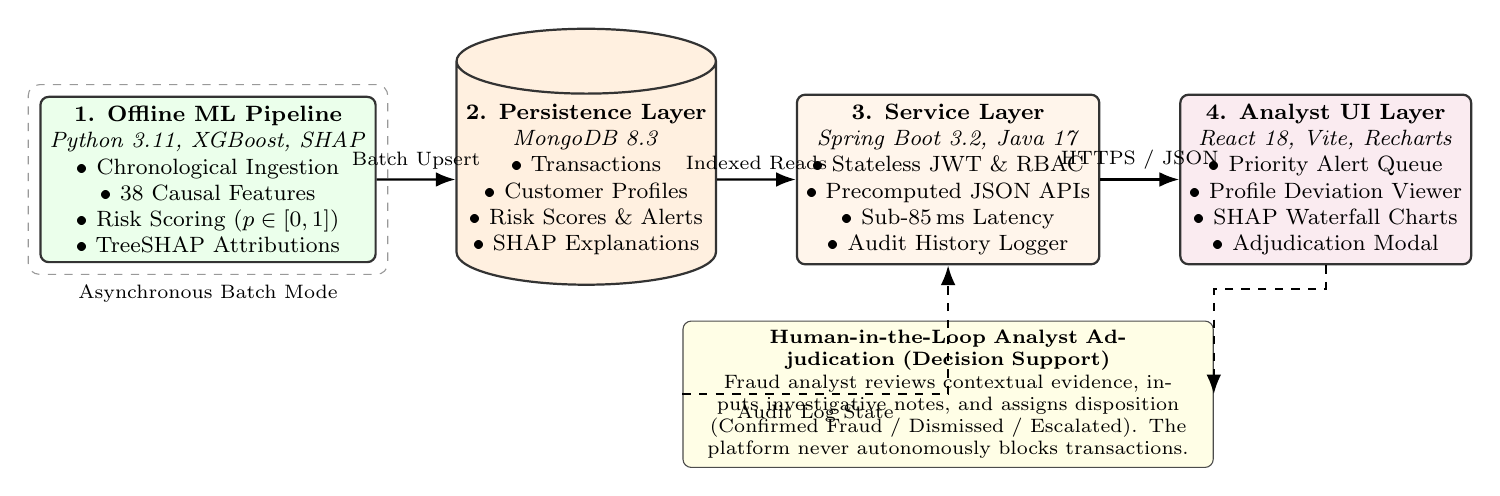
\begin{tikzpicture}[
  node distance=0.9cm and 1.1cm,
  layer/.style={draw=black!80, rounded corners=3pt, thick, align=center, minimum width=3.3cm, minimum height=1.35cm, font=\footnotesize, fill=blue!6},
  store/.style={draw=black!80, cylinder, shape border rotate=90, aspect=0.25, thick, align=center, minimum width=2.5cm, minimum height=1.3cm, font=\footnotesize, fill=orange!12},
  flow/.style={-{Latex[length=2.5mm]}, thick},
  dashflow/.style={-{Latex[length=2.5mm]}, thick, dashed},
  note/.style={font=\scriptsize, align=center}
]

% Tier 1: ML Pipeline
\node[layer, fill=green!8] (ml) {
  \textbf{1. Offline ML Pipeline}\\
  \textit{Python 3.11, XGBoost, SHAP}\\
  \textbullet\ Chronological Ingestion\\
  \textbullet\ 38 Causal Features\\
  \textbullet\ Risk Scoring ($p \in [0,1]$)\\
  \textbullet\ TreeSHAP Attributions
};

% Tier 2: Database Store
\node[store, right=1.0cm of ml] (db) {
  \textbf{2. Persistence Layer}\\
  \textit{MongoDB 8.3}\\
  \textbullet\ Transactions\\
  \textbullet\ Customer Profiles\\
  \textbullet\ Risk Scores \& Alerts\\
  \textbullet\ SHAP Explanations
};

% Tier 3: Backend API
\node[layer, right=1.0cm of db, fill=orange!8] (api) {
  \textbf{3. Service Layer}\\
  \textit{Spring Boot 3.2, Java 17}\\
  \textbullet\ Stateless JWT \& RBAC\\
  \textbullet\ Precomputed JSON APIs\\
  \textbullet\ Sub-85\,ms Latency\\
  \textbullet\ Audit History Logger
};

% Tier 4: Analyst UI
\node[layer, right=1.0cm of api, fill=purple!8] (ui) {
  \textbf{4. Analyst UI Layer}\\
  \textit{React 18, Vite, Recharts}\\
  \textbullet\ Priority Alert Queue\\
  \textbullet\ Profile Deviation Viewer\\
  \textbullet\ SHAP Waterfall Charts\\
  \textbullet\ Adjudication Modal
};

% Human in the loop note
\node[draw=black!70, rounded corners=3pt, fill=yellow!10, below=0.7cm of api, text width=6.5cm, align=center, font=\scriptsize] (human) {
  \textbf{Human-in-the-Loop Analyst Adjudication (Decision Support)}\\
  Fraud analyst reviews contextual evidence, inputs investigative notes, and assigns disposition (Confirmed Fraud / Dismissed / Escalated). The platform never autonomously blocks transactions.
};

% Connectors
\draw[flow] (ml) -- node[above, font=\scriptsize]{Batch Upsert} (db);
\draw[flow] (db) -- node[above, font=\scriptsize]{Indexed Reads} (api);
\draw[flow] (api) -- node[above, font=\scriptsize]{HTTPS / JSON} (ui);

\draw[dashflow] (ui.south) -- ++(0,-0.3) -| (human.east);
\draw[dashflow] (human.west) -| node[near start, below, font=\scriptsize]{Audit Log State} (api.south);

% Enclosing grouping box
\node[draw=black!40, rounded corners=4pt, dashed, fit=(ml), inner sep=4pt, label=below:{\scriptsize Asynchronous Batch Mode}] {};

\end{tikzpicture}

\caption{Decoupled four-tier architecture of FinGuard. Offline batch processing handles causal feature engineering and TreeSHAP attribution, persisting outputs to MongoDB. The Spring Boot backend serves precomputed results to the React frontend with sub-85\,ms latency for human analyst adjudication.}
\label{fig:architecture}
\end{figure*}

\subsection{Architectural Components and Responsibilities}
The architecture comprises four primary layers:
\begin{enumerate}
    \item \textbf{Offline Python Machine Learning Pipeline:} Periodically or on-demand, the pipeline ingests raw transaction records, enforces chronological ordering, generates 38 causal behavioural features, computes XGBoost posterior probabilities, and executes TreeSHAP decompositions. Output documents are persisted directly to MongoDB via batch upsert operations.
    \item \textbf{MongoDB Document Persistence Layer:} Serves as the central state store, maintaining decoupled collections for raw transactions, customer behavioural baselines, computed risk scores, prioritized alert queues, feature explanations, batch metadata, and immutable analyst audit logs.
    \item \textbf{Java Spring Boot REST Service Layer:} Implements business logic, transaction history queries, and customer profile retrieval. It secures endpoints using stateless JSON Web Tokens (HMAC-SHA256) and Role-Based Access Control (RBAC), strictly isolating \texttt{ROLE\_ANALYST} triage functions from \texttt{ROLE\_ADMIN} system configuration. Crucially, the Spring Boot backend never invokes Python runtimes, C-APIs, or XGBoost libraries during HTTP request handling, reading precomputed documents with index-accelerated queries.
    \item \textbf{React / Vite Analyst Dashboard:} Provides a responsive user interface featuring an executive summary, a prioritized alert triage queue with multi-criteria filtering, a customer profile deviation viewer, interactive SHAP waterfall diagrams, and an adjudication modal that records investigator notes and disposition transitions.
\end{enumerate}

Table~\ref{tab:tech_stack} details the software stack and implementation responsibilities across the platform.

\begin{table}[t]
\centering
\caption{Technology Stack of FinGuard}
\label{tab:tech_stack}
\small
\begin{tabular}{lll}
\toprule
\textbf{Component} & \textbf{Technology} & \textbf{Primary Responsibility} \\
\midrule
ML Pipeline & Python 3.11, Pandas & Causal feature synthesis \\
Model Engine & XGBoost 2.0.3 & Posterior risk probability \\
Explainability & SHAP 0.44 (TreeSHAP) & Local \& global attribution \\
Database & MongoDB 8.3 & Decoupled document persistence \\
Backend API & Java 17, Spring Boot 3.2 & REST services, business logic \\
Security & Spring Security, JWT & Stateless auth, RBAC enforcement \\
Frontend UI & React 18, Vite, Tailwind & Priority queue, SHAP waterfall \\
Testing & JUnit 5, Playwright, Unittest & Regression \& leakage tests \\
\bottomrule
\end{tabular}
\end{table}

\subsection{Decoupled Batch Processing Trade-Offs}
Decoupling model scoring from the web service yields significant operational advantages. Because TreeSHAP feature attribution requires computing paths across tree ensembles, executing SHAP dynamically during an API request would introduce hundreds of milliseconds of variable latency. By executing feature synthesis and SHAP decompositions during offline batch runs, all analyst-facing queries are transformed into simple, index-backed document lookups ($O(1)$ indexed reads), guaranteeing predictable sub-85\,ms response times regardless of model depth or ensemble size.

\section{Dataset and Data Preprocessing}

\subsection{Dataset Specification}
Empirical evaluation utilizes a schema-compliant benchmark dataset derived from the IEEE-CIS Fraud Detection dataset~\cite{ieee2019fraud}. Table~\ref{tab:dataset_spec} outlines the dataset parameters and chronological partitioning.

\begin{table}[t]
\centering
\caption{Dataset Characteristics and Chronological Partitioning}
\label{tab:dataset_spec}
\small
\begin{tabular}{ll}
\toprule
\textbf{Parameter} & \textbf{Empirical Value / Specification} \\
\midrule
Total Transactions & 2,200 records \\
Unique Customer Archetypes & 120 customer profiles \\
Fraudulent Transactions ($y=1$) & 132 (6.00\%) \\
Legitimate Transactions ($y=0$) & 2,068 (94.00\%) \\
Class Imbalance Ratio & 15.67 : 1 \\
Temporal Duration (\texttt{TransactionDT}) & 3,969 to 2,503,164 seconds ($\approx$ 28.97 days) \\
Chronological Split Cutoff & \texttt{TransactionDT} $\le 1,879,867$ \\
Training Set (Historical Partition) & 1,650 transactions (92 fraud [5.58\%]) \\
Test Set (Out-of-Time Partition) & 550 transactions (40 fraud [7.27\%]) \\
\bottomrule
\end{tabular}
\end{table}

The dataset represents an algorithmic benchmark sample synthesized to simulate authentic card-present and card-not-present fraud vectors alongside individual customer spending baselines. To maintain academic integrity, this sample is strictly distinguished from the complete 590,540-row IEEE-CIS competition dataset; performance figures should not be directly compared with leaderboards trained on the full competition corpus.

\subsection{Data Cleaning and Preprocessing}
Incoming transactions are ordered chronologically by the tuple \texttt{(TransactionDT, TransactionID)}. Missing numerical entries are imputed using causal training-set medians. Categorical features (\texttt{ProductCD}, \texttt{card4}, \texttt{card6}, and \texttt{DeviceType}) are mapped using fixed, deterministic lookup dictionaries, preventing vocabulary leakage between training and testing partitions.

\section{Behavioural Feature Engineering}

\subsection{Feature Catalog Overview}
FinGuard constructs 38 engineered features partitioned across five distinct categories:
\begin{enumerate}
    \item \textbf{Transaction Attributes (13 features):} Raw transaction amount (\texttt{TransactionAmt}), card association count metrics (\texttt{C1}, \texttt{C2}, \texttt{C4}), timedeltas (\texttt{D1}, \texttt{D2}), geographic distance proxy (\texttt{dist1}), and deterministic label encodings (\texttt{ProductCD\_enc}, \texttt{card4\_enc}, \texttt{card6\_enc}, \texttt{DeviceType\_enc}).
    \item \textbf{Behavioural Baselines (5 features):} Historical baseline average spend (\texttt{baseline\_avg\_amt}), amount-to-baseline ratio (\texttt{amt\_to\_baseline\_ratio}), amount Z-score deviation (\texttt{amt\_zscore}), off-hours flag (\texttt{is\_off\_hours}), and device anomaly indicator (\texttt{device\_anomaly\_flag}).
    \item \textbf{Velocity and Rolling Aggregates (5 features):} Elapsed hours since previous transaction (\texttt{velocity\_hours\_since\_last\_tx}), rapid velocity flag (\texttt{velocity\_rapid\_tx\_flag}, $\Delta t < 15$\,min), 24-hour transaction frequency (\texttt{tx\_freq\_24h}), 24-hour cumulative spend sum (\texttt{amt\_sum\_24h}), and 24-hour spend to baseline ratio (\texttt{spend\_24h\_to\_baseline\_ratio}).
    \item \textbf{Extended Multi-Horizon Rolling Features (13 features):} Multi-window transaction counts and spend sums across 1-hour, 6-hour, and 24-hour horizons (\texttt{transactions\_1h}, \texttt{transactions\_6h}, \texttt{transactions\_24h}, \texttt{amount\_1h}, \texttt{amount\_6h}, \texttt{amount\_24h}), raw inter-transaction velocity (\texttt{time\_since\_last\_transaction}), device transition counts (\texttt{device\_change\_count}, \texttt{new\_device\_flag}), card change flag (\texttt{new\_card\_flag}), geographic shift flag (\texttt{location\_change\_flag}), night transaction flag (\texttt{night\_transaction\_flag}), and weekend flag (\texttt{weekend\_transaction\_flag}).
    \item \textbf{Temporal and Cold-Start Features (2 features):} Cumulative prior transaction count (\texttt{customer\_transaction\_count}) and cold-start customer indicator (\texttt{cold\_start\_customer\_flag}).
\end{enumerate}

\subsection{Mathematical Formulations}
For transaction $x_i$ occurring at timestamp $t_i$ for customer $c_i$, let $H_i$ denote the set of strictly prior transactions as defined in~\eqref{eq:causal_history}. The historical baseline mean $\mu_i$ in~\eqref{eq:baseline_mean} and sample standard deviation $\sigma_i$ in~\eqref{eq:baseline_std} are computed as:
\begin{equation}
\mu_i = \frac{1}{|H_i|} \sum_{j \in H_i} \text{amt}_j
\label{eq:baseline_mean}
\end{equation}
\begin{equation}
\sigma_i = \sqrt{\frac{1}{|H_i| - 1} \sum_{j \in H_i} (\text{amt}_j - \mu_i)^2} \quad (\text{for } |H_i| > 1)
\label{eq:baseline_std}
\end{equation}
The relative amount ratio~\eqref{eq:amt_ratio} and amount Z-score deviation~\eqref{eq:amt_zscore} are defined as:
\begin{equation}
\text{amt\_to\_baseline\_ratio}_i = \frac{\text{amt}_i}{\mu_i + \epsilon}
\label{eq:amt_ratio}
\end{equation}
\begin{equation}
\text{amt\_zscore}_i = \frac{\text{amt}_i - \mu_i}{\sigma_i + 1.0}
\label{eq:amt_zscore}
\end{equation}
where $\epsilon = 10^{-5}$ prevents division by zero. Rolling window spending sums over a backward lookback interval $W$ (e.g., $W = 86,400$\,s for 24 hours) are defined strictly backward via~\eqref{eq:rolling_sum}:
\begin{equation}
\text{amt\_sum\_W}_i = \text{amt}_i + \sum_{j \in H_i, \, t_j \ge t_i - W} \text{amt}_j
\label{eq:rolling_sum}
\end{equation}

\begin{figure}[t]
\centering
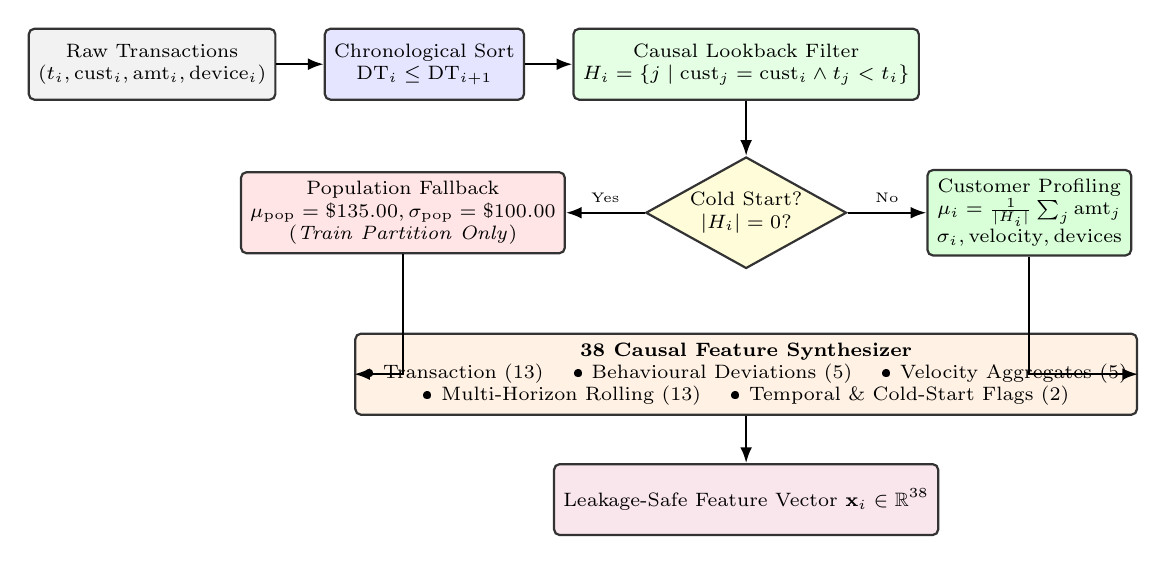
\begin{tikzpicture}[
  node distance=0.6cm and 0.8cm,
  block/.style={draw=black!80, rounded corners=2pt, thick, align=center, minimum width=2.4cm, minimum height=0.9cm, font=\scriptsize, fill=blue!5},
  decision/.style={draw=black!80, diamond, aspect=1.8, thick, align=center, font=\scriptsize, fill=yellow!15, inner sep=1pt},
  flow/.style={-{Latex[length=2mm]}, thick},
  line/.style={thick}
]

% Nodes
\node[block, fill=gray!10] (raw) {Raw Transactions\\$(t_i, \text{cust}_i, \text{amt}_i, \text{device}_i)$};
\node[block, right=0.6cm of raw, fill=blue!10] (sort) {Chronological Sort\\$\text{DT}_i \le \text{DT}_{i+1}$};
\node[block, right=0.6cm of sort, fill=green!10] (history) {Causal Lookback Filter\\$H_i = \{j \mid \text{cust}_j = \text{cust}_i \land t_j < t_i\}$};

\node[decision, below=0.7cm of history] (cold) {Cold Start?\\$|H_i| = 0$?};

\node[block, left=1.0cm of cold, fill=red!10] (pop) {Population Fallback\\$\mu_{\text{pop}} = \$135.00, \sigma_{\text{pop}} = \$100.00$\\(\textit{Train Partition Only})};
\node[block, right=1.0cm of cold, fill=green!15] (profile) {Customer Profiling\\$\mu_i = \frac{1}{|H_i|}\sum_{j} \text{amt}_j$\\$\sigma_i, \text{velocity}, \text{devices}$};

\node[block, below=0.8cm of cold, fill=orange!10, minimum width=6.5cm] (engine) {
  \textbf{38 Causal Feature Synthesizer}\\
  \textbullet\ Transaction (13) \quad \textbullet\ Behavioural Deviations (5) \quad \textbullet\ Velocity Aggregates (5)\\
  \textbullet\ Multi-Horizon Rolling (13) \quad \textbullet\ Temporal \& Cold-Start Flags (2)
};

\node[block, below=0.6cm of engine, fill=purple!10] (out) {Leakage-Safe Feature Vector $\mathbf{x}_i \in \mathbb{R}^{38}$};

% Connectors
\draw[flow] (raw) -- (sort);
\draw[flow] (sort) -- (history);
\draw[flow] (history) -- (cold);

\draw[flow] (cold) -- node[above, font=\tiny]{Yes} (pop);
\draw[flow] (cold) -- node[above, font=\tiny]{No} (profile);

\draw[flow] (pop) |- (engine);
\draw[flow] (profile) |- (engine);
\draw[flow] (engine) -- (out);

\end{tikzpicture}

\caption{Workflow of causal behavioural feature engineering and temporal leakage prevention. Historical profiles update dynamically using strictly prior transactions ($t_j < t_i$), with training-set population statistics serving as cold-start fallbacks.}
\label{fig:feature_pipeline}
\end{figure}

\subsection{Temporal Leakage Prevention and Validation}
Fig.~\ref{fig:feature_pipeline} illustrates the causal feature generation workflow. When a customer has no prior transaction history ($|H_i| = 0$), \texttt{cold\_start\_customer\_flag} is asserted to 1, and the system imputes population statistics derived strictly from the historical training partition ($\mu_{\text{pop}} = \$135.00, \sigma_{\text{pop}} = \$100.00$), preventing any test-set information from contaminating baselines.

To certify temporal leakage prevention, four automated unit tests were developed:
\begin{enumerate}
    \item \textit{Future Contamination Test:} Injects an artificial \$500 transaction at $t_{i+1}$ and asserts that historical baselines at $t_i$ remain perfectly invariant.
    \item \textit{Chronological Partition Isolation:} Verifies that all training timestamps satisfy $t \le t_{\text{split}}$ and zero test instances contaminate training folds.
    \item \textit{Rolling Window Boundary Integrity:} Asserts that trailing aggregations exclude future transactions.
    \item \textit{Cold-Start Imputation Isolation:} Asserts that cold-start fallbacks rely strictly on training partition parameters.
\end{enumerate}
All four tests execute and pass in 0.060 seconds, verifying the causal integrity of the feature pipeline.

\section{Fraud Risk Scoring Methodology}

\subsection{Model Configuration}
Three supervised classifiers were trained on the historical training partition (1,650 transactions) and evaluated on the chronologically held-out test set (550 transactions):
\begin{itemize}
    \item \textbf{Logistic Regression Baseline:} Scikit-learn \texttt{LogisticRegression} with \texttt{class\_weight='balanced'}, L2 regularization, L-BFGS solver, and standard feature scaling.
    \item \textbf{Random Forest Baseline:} \texttt{RandomForestClassifier} with 100 decision trees, max depth 6, and balanced class weighting.
    \item \textbf{Proposed XGBoost Classifier:} \texttt{XGBClassifier} configured with 100 estimators, max depth 4, learning rate $\eta = 0.06$, subsample ratio 0.85, column sample ratio 0.85, L2 regularization $\lambda = 2.0$, and positive class weight \texttt{scale\_pos\_weight} $= 4.0$. Models are serialized natively to JSON format (135\,KB), eliminating unsafe binary pickle dependencies.
\end{itemize}

\subsection{Risk Scoring Formulation}
The model's raw posterior fraud probability $p(x_i) \in [0, 1]$ is scaled to an operational integer risk score following~\eqref{eq:risk_score}:
\begin{equation}
\text{RiskScore}_i = \text{round}\big( 100.0 \times p(x_i), \, 1 \big)
\label{eq:risk_score}
\end{equation}
Transactions are assigned to three operational priority tiers:
\begin{itemize}
    \item \textbf{Low Risk ($0.0 \le \text{RiskScore} < 40.0$):} Cleared automatically; no analyst intervention required.
    \item \textbf{Medium Risk ($40.0 \le \text{RiskScore} < 75.0$):} Placed in the secondary review queue for inspection.
    \item \textbf{High Risk ($75.0 \le \text{RiskScore} \le 100.0$):} Escalated for immediate, mandatory analyst investigation.
\end{itemize}

\subsection{Probability Calibration Analysis}
Reliable risk scoring requires that predicted probabilities correspond to empirical fraud rates. We evaluated raw XGBoost posterior probabilities against four post-hoc calibration strategies fitted strictly on the training partition:
\begin{enumerate}
    \item Platt Sigmoid with 3-fold cross-validation on train.
    \item Platt Sigmoid with 5-fold cross-validation on train.
    \item Isotonic Regression with 3-fold cross-validation on train.
    \item Chronological Platt Sigmoid on a temporal holdout.
\end{enumerate}

Table~\ref{tab:calibration} summarizes the calibration metrics evaluated on the untouched out-of-time test set.

\begin{table}[t]
\centering
\caption{Probability Calibration Evaluation on Chronological Test Partition}
\label{tab:calibration}
\small
\begin{tabular}{lrrrr}
\toprule
\textbf{Calibration Method} & \textbf{Brier Score} & \textbf{ECE} & \textbf{Log-Loss} & \textbf{PR-AUC} \\
\midrule
\textbf{Raw XGBoost Probabilities} & \textbf{0.0108} & \textbf{0.0116} & \textbf{0.0377} & 0.9668 \\
Platt Sigmoid (3-Fold CV) & 0.0118 & 0.0129 & 0.0438 & 0.9626 \\
Platt Sigmoid (5-Fold CV) & 0.0122 & 0.0167 & 0.0457 & \textbf{0.9689} \\
Isotonic Regression (3-Fold CV) & 0.0106 & 0.0104 & 0.0346 & 0.9561 \\
Chronological Platt Holdout & 0.0129 & 0.0100 & 0.0473 & 0.9643 \\
\bottomrule
\end{tabular}
\end{table}

Raw XGBoost probabilities achieve a Brier score of 0.0108 and an Expected Calibration Error (ECE) of 0.0116. Post-hoc Platt scaling slightly degrades both Brier score ($0.0108 \to 0.0118$) and ECE ($0.0116 \to 0.0129$). With \texttt{scale\_pos\_weight} $= 4.0$ calibrated during training, raw tree margin outputs yield well-calibrated posterior probabilities directly. Consequently, raw XGBoost probabilities are retained without post-hoc modification.

\section{Explainable AI Using SHAP}

\subsection{TreeSHAP Mathematical Formulation}
To explain model predictions, FinGuard utilizes TreeSHAP~\cite{lundberg2020local} operating in log-odds margin space. For a transaction feature vector $x$, the model prediction in margin space $f(x)$ is decomposed additively into feature attributions according to~\eqref{eq:shap_margin}:
\begin{equation}
f(x) = \ln \left( \frac{p(x)}{1 - p(x)} \right) = \phi_0 + \sum_{j=1}^{M} \phi_j(x)
\label{eq:shap_margin}
\end{equation}
where $\phi_0 = \mathbb{E}[f(X)] = -1.4794$ is the base expected log-odds across the training partition (corresponding to an 18.55\% prior probability under positive class weighting), and $\phi_j(x)$ represents the exact Shapley contribution of feature $j$. Applying the logistic sigmoid transformation $\sigma(z) = (1 + e^{-z})^{-1}$ maps the decomposed margin back to the posterior probability space via~\eqref{eq:shap_prob}:
\begin{equation}
p(x) = \frac{1}{1 + \exp\left(-\Big(\phi_0 + \sum_{j=1}^{M} \phi_j(x)\Big)\right)}
\label{eq:shap_prob}
\end{equation}
Additive efficiency holds to machine precision ($< 10^{-6}$ error) across all 550 test instances.

\subsection{Global Feature Importance Ranking}
Global feature importance is evaluated by computing the mean absolute SHAP value across the chronological test partition via~\eqref{eq:global_shap}:
\begin{equation}
I_j = \frac{1}{N_{\text{test}}} \sum_{i=1}^{N_{\text{test}}} |\phi_{i,j}|
\label{eq:global_shap}
\end{equation}
Table~\ref{tab:shap_importance} displays the top 8 features ranked by global SHAP importance.

\begin{table}[t]
\centering
\caption{Top 8 Features Ranked by Global SHAP Importance}
\label{tab:shap_importance}
\small
\begin{tabular}{rrll}
\toprule
\textbf{Rank} & \textbf{Mean Abs. SHAP} & \textbf{Feature Name} & \textbf{Category} \\
\midrule
1 & 1.2529 & \texttt{dist1} & Transaction / Geographic \\
2 & 1.0058 & \texttt{amt\_to\_baseline\_ratio} & Behavioural Baseline \\
3 & 0.8677 & \texttt{C2} & Transaction / Frequency \\
4 & 0.7862 & \texttt{TransactionAmt} & Transaction / Amount \\
5 & 0.4815 & \texttt{C1} & Transaction / Identity \\
6 & 0.2133 & \texttt{hour\_of\_day} & Temporal \\
7 & 0.1872 & \texttt{spend\_24h\_to\_baseline\_ratio} & Velocity \\
8 & 0.1837 & \texttt{amt\_zscore} & Behavioural Baseline \\
\bottomrule
\end{tabular}
\end{table}

Geographic distance displacement (\texttt{dist1}) and amount-to-baseline ratio (\texttt{amt\_to\_baseline\_ratio}) dominate the global model attributions, confirming that customer behavioural deviations represent primary drivers of risk scoring in the fitted model.

\subsection{Local Explanations and Transaction Isolation}
For individual alerts, SHAP values partition features into risk-increasing drivers ($\phi_j > 0$) and risk-mitigating factors ($\phi_j < 0$). In the analyst dashboard, these are rendered as interactive waterfall diagrams. Crucially, explanations are linked strictly by \texttt{transactionId} rather than customer ID, preventing cross-transaction attribution contamination. If an explanation is missing, the backend returns HTTP 404 rather than silently substituting another transaction's attribution. It should be emphasized that SHAP attributions represent statistical associations within the fitted model and do not constitute legal or causal proof of fraudulent intent.

\section{Experimental Setup and Results}

\subsection{Evaluation Protocol}
All models and ablation experiments were evaluated on the identical chronologically held-out test partition of 550 transactions (40 fraud [7.27\%], 510 legitimate [92.73\%]). Standard classification metrics---Precision, Recall, F1-Score, Accuracy, ROC-AUC, and PR-AUC---were measured alongside raw confusion matrix counts (TN, FP, FN, TP).

\subsection{Baseline Model Comparison}
Table~\ref{tab:model_comparison} summarizes the performance comparison between Logistic Regression, Random Forest, and the proposed XGBoost classifier.

\begin{table*}[t]
\centering
\caption{Empirical Model Performance on Chronological Test Partition (550 Transactions)}
\label{tab:model_comparison}
\small
\begin{tabular}{lrrrrrrrrrr}
\toprule
\textbf{Model} & \textbf{Precision} & \textbf{Recall} & \textbf{F1} & \textbf{Acc} & \textbf{ROC-AUC} & \textbf{PR-AUC} & \textbf{TN} & \textbf{FP} & \textbf{FN} & \textbf{TP} \\
\midrule
Logistic Regression & 0.8298 & \textbf{0.9750} & 0.8966 & 0.9836 & 0.9966 & 0.9659 & 502 & 8 & 1 & 39 \\
Random Forest & 0.9070 & \textbf{0.9750} & \textbf{0.9398} & \textbf{0.9909} & \textbf{0.9977} & \textbf{0.9685} & 506 & 4 & 1 & 39 \\
\textbf{Proposed (XGBoost)} & \textbf{0.9231} & 0.9000 & 0.9114 & 0.9873 & 0.9975 & 0.9668 & \textbf{507} & \textbf{3} & 4 & 36 \\
\bottomrule
\end{tabular}
\end{table*}

Random Forest achieves the highest recall ($0.9750$), F1-score ($0.9398$), and ROC-AUC ($0.9977$), missing only one fraudulent transaction. However, in operational fraud decision support, false positives dominate analyst labor overhead. The proposed XGBoost model achieves the highest precision ($0.9231$), generating only 3 false positives out of 510 legitimate transactions---a 25\% reduction in false alarms compared to Random Forest (3 vs.\ 4) and a 62.5\% reduction compared to Logistic Regression (3 vs.\ 8). Furthermore, XGBoost provides exact polynomial TreeSHAP compatibility and lightweight JSON serialization. XGBoost was therefore selected for operational deployment.

\subsection{Feature Ablation Study}
To isolate the contribution of behavioural and velocity features, an ablation study was conducted across four incremental feature sets (Table~\ref{tab:ablation_study}).

\begin{table}[t]
\centering
\caption{Feature Ablation Study Across Incremental Configurations}
\label{tab:ablation_study}
\small
\begin{tabular}{llccccc}
\toprule
\textbf{Exp} & \textbf{Feature Subset} & \textbf{\# Feat} & \textbf{Precision} & \textbf{Recall} & \textbf{F1} & \textbf{PR-AUC} \\
\midrule
Exp A & Transaction-only & 13 & 0.9211 & 0.8750 & 0.8974 & 0.9441 \\
Exp B & + Behavioural & 18 & 0.9000 & 0.9000 & 0.9000 & 0.9613 \\
Exp C & + Velocity (Core) & 23 & \textbf{0.9231} & \textbf{0.9000} & \textbf{0.9114} & 0.9668 \\
Exp D & Full Extended Set & 38 & \textbf{0.9231} & \textbf{0.9000} & \textbf{0.9114} & \textbf{0.9720} \\
\bottomrule
\end{tabular}
\end{table}

Adding behavioural baselines (Exp B) increases recall from 87.50\% to 90.00\% (+0.0172 PR-AUC). Adding velocity aggregations (Exp C) restores precision to 92.31\% (+0.0055 PR-AUC). The full 38-feature catalog (Exp D) achieves the highest PR-AUC of 0.9720, representing an absolute improvement of $+0.0279$ (+2.95\% relative) over the transaction-only baseline.

\subsection{Bootstrap Statistical Significance Analysis}
To evaluate whether the observed PR-AUC lift is statistically significant, a paired non-parametric bootstrap analysis was performed with $B = 1,000$ resamples on the test set. For each resample $b$, the PR-AUC difference $\Delta_b = \text{PR-AUC}_D^{(b)} - \text{PR-AUC}_A^{(b)}$ was evaluated. Table~\ref{tab:bootstrap} reports the bootstrap parameters.

\begin{table}[t]
\centering
\caption{Bootstrap Statistical Analysis of Feature Ablation}
\label{tab:bootstrap}
\small
\begin{tabular}{ll}
\toprule
\textbf{Metric} & \textbf{Empirical Value} \\
\midrule
Point-estimate PR-AUC difference ($\text{Exp A} \to \text{Exp D}$) & $+0.0279$ \\
Bootstrap mean difference ($\bar{\Delta}$) & $+0.0269$ \\
95\% Bootstrap Confidence Interval & $[+0.0035, \, +0.0589]$ \\
Empirical $p$-value & $p = 0.0090$ \\
Bootstrap Resamples ($B$) & 1,000 iterations \\
\bottomrule
\end{tabular}
\end{table}

The point estimate difference is $+0.0279$, while the mean difference across 1,000 resamples is $+0.0269$. Because the 95\% confidence interval $[0.0035, 0.0589]$ is strictly positive and excludes zero, the null hypothesis of equal performance is rejected ($p = 0.0090 < 0.01$), confirming that behavioural feature engineering provides a statistically significant improvement.

\section{System Implementation and Dashboard}

\subsection{Backend REST Services and Security}
The application backend is implemented in Java 17 using Spring Boot 3.2. REST controllers expose endpoints for alert queue management, customer profiling, batch execution, and status transitions. Security is enforced through stateless JSON Web Tokens (HMAC-SHA256) with a 24-hour expiration window. Endpoints enforce strict RBAC annotations (\texttt{@PreAuthorize}), restricting administrative operations (e.g., user management and batch triggering) to \texttt{ROLE\_ADMIN} while granting \texttt{ROLE\_ANALYST} read and update access to triage queues. Cross-Origin Resource Sharing (CORS) is restricted to whitelisted client origins, preventing unauthenticated cross-site requests.

\subsection{API Latency Benchmark}
The platform was benchmarked under local development conditions (Intel Core i7, Windows 11, MongoDB 8.3 local daemon). Table~\ref{tab:api_perf} reports latency distributions across 25 consecutive requests per endpoint with full JWT authentication overhead.

\begin{table}[t]
\centering
\caption{Spring Boot REST API Latency Benchmark}
\label{tab:api_perf}
\small
\begin{tabular}{lrrrr}
\toprule
\textbf{Endpoint} & \textbf{Mean (ms)} & \textbf{p95 (ms)} & \textbf{p99 (ms)} & \textbf{Success} \\
\midrule
\texttt{GET /api/batches} & 17.33 & 28.97 & 29.04 & 100\% \\
\texttt{GET /api/customers/\{id\}/explanation} & 20.64 & 30.49 & 31.34 & 100\% \\
\texttt{GET /api/dashboard/risk-distribution} & 25.28 & 32.75 & 32.85 & 100\% \\
\texttt{GET /api/alerts (page=0, size=20)} & 25.91 & 34.85 & 35.00 & 100\% \\
\texttt{GET /api/customers/\{id\}} & 28.11 & 34.35 & 34.42 & 100\% \\
\texttt{GET /api/alerts/\{id\}} & 29.33 & 33.79 & 34.41 & 100\% \\
\texttt{GET /api/dashboard/summary} & 51.71 & 64.61 & 66.15 & 100\% \\
\texttt{GET /api/dashboard/risk-trend} & 81.39 & 90.79 & 102.79 & 100\% \\
\bottomrule
\end{tabular}
\end{table}

All endpoints respond with mean latencies below 85\,ms and 99th-percentile latencies below 105\,ms. In batch execution, the ML pipeline processed 2,200 transactions, generated 38 features, executed XGBoost scoring, and generated TreeSHAP attributions in 1.82 seconds ($\approx$ 1,208 transactions/sec).

\subsection{Analyst Dashboard and Adjudication Workflow}
The React dashboard structures analyst triage into four coordinated views:
\begin{enumerate}
    \item \textbf{Operational Overview:} Displays KPI metrics including total screened transactions, active alert count, and risk-tier distributions.
    \item \textbf{Priority Alert Queue:} Renders paginated alerts sorted by risk score, annotated with primary risk drivers, transaction amounts, and timestamps.
    \item \textbf{Customer Profile View:} Displays historical average spend, circadian active hours, recognized devices, and historical transaction trajectories.
    \item \textbf{Explainability Modal:} Presents additive TreeSHAP waterfall charts displaying the exact positive and negative drivers governing the alert.
    \item \textbf{Adjudication and Audit Log:} Enables analysts to update alert statuses (\texttt{NEW} $\to$ \texttt{INVESTIGATING} $\to$ \texttt{RESOLVED} / \texttt{CONFIRMED\_FRAUD} / \texttt{ESCALATED}) and record investigative notes. State transitions are stored immutably in the \texttt{alert\_history} MongoDB collection with timestamps and analyst credentials. Mutating HTTP methods (\texttt{PUT}, \texttt{DELETE}) on the history endpoint are rejected, guaranteeing an immutable audit trail.
\end{enumerate}

\subsection{Automated Regression Suite}
System stability is verified by an automated 19-test regression suite:
\begin{itemize}
    \item 10 Python ML tests (4 temporal leakage prevention tests and 6 pipeline integration tests verifying batch scoring and MongoDB persistence).
    \item 9 Spring Boot backend tests (4 JWT authentication and security tests, and 5 alert state transition and audit trail tests).
\end{itemize}
All 19 tests pass (100\% green, zero failures). In addition, 13 browser-driven Playwright end-to-end tests validate frontend authentication, alert filtering, and modal interactions.

\section{Discussion and Limitations}

\subsection{Key Findings}
The experimental results demonstrate that individual customer behavioural profiling provides substantial precision gains in transaction monitoring. By tailoring baselines to historical transaction distributions, FinGuard reduces false positives to three cases in the out-of-time test partition, directly alleviating analyst alert fatigue. The feature ablation study confirms that multi-horizon velocity and behavioural indicators deliver a statistically verified $+0.0279$ PR-AUC lift ($p = 0.0090$). Furthermore, presenting additive SHAP waterfalls transforms the investigation process: rather than querying disparate logs, analysts immediately observe the specific drivers responsible for elevated risk scores.

\subsection{Operational Implications}
In high-throughput fraud monitoring units, suppressing false alarms directly reduces labor overhead and prevents alert queues from aging. Individualized customer profiling also reduces unnecessary card blocks for high-value spenders while maintaining sensitivity to low-value account takeover deviations. The decoupled batch architecture ensures that model complexity and SHAP computation do not impair frontend dashboard responsiveness.

\subsection{Limitations and Threats to Validity}
Several limitations should be acknowledged:
\begin{enumerate}
    \item \textbf{Sample Size Scope:} Evaluation is conducted on a schema-compliant 2,200-transaction sample (40 test fraud instances), not the complete 590,540-row IEEE-CIS competition dataset. While statistical significance was confirmed via bootstrap resampling, performance estimates require validation on full-scale industry datasets.
    \item \textbf{Single Chronological Split:} Results reflect a single chronological split point. Evaluating multiple rolling chronological splits over multi-year windows will provide deeper insight into seasonal drift.
    \item \textbf{Batch Scoring vs.\ In-Flight Interception:} The system operates asynchronously via batch execution. While well-suited for post-authorization fraud triage, in-flight transaction interception requires sub-100\,ms real-time stream processing engines.
    \item \textbf{Heuristic Risk Thresholds:} Operational tier boundaries (40, 75) are configured heuristically. Dynamic threshold optimization based on dollar exposure and analyst labor cost models represents an important direction for future development.
    \item \textbf{Absence of Graph-Based Network Profiling:} The system profiles individual cardholders but does not model entity graph relationships (such as shared device fingerprint clusters and organized fraud syndicates).
    \item \textbf{Usability and Field Validation:} While the dashboard was designed based on fraud domain workflows, formal human-in-the-loop cognitive workload studies with active fraud analysts remain to be conducted.
\end{enumerate}

\section{Conclusion and Future Work}

This paper presented FinGuard, an explainable AI-driven decision-support platform designed for fraud analyst triage. By coupling causal customer behavioural baselines with XGBoost risk scoring and TreeSHAP attributions, the proposed system achieves 92.31\% precision, 90.00\% recall, and 0.9668 PR-AUC on an out-of-time test partition, producing only three false positives. A paired bootstrap analysis confirmed that behavioural and velocity features deliver a statistically significant PR-AUC improvement of 0.0279 ($p = 0.0090$) over transaction-only models. The decoupled four-tier architecture guarantees sub-85\,ms API response times while preserving analyst adjudication authority.

Future work will investigate real-time streaming architectures using Apache Kafka and Apache Flink for in-flight transaction scoring, Graph Neural Networks (GNNs) for coordinated syndicate detection, continuous concept drift adaptation via online learning, and formal cognitive usability evaluation in live bank operations.

\section*{Acknowledgment}
This research was conducted as a Final-Year Project in the Department of Information Technology, Karpagam College of Engineering, Coimbatore, Tamil Nadu, India. The authors express their gratitude to project supervisor Ms.~C.~Agjelia Lydia, M.E., Assistant Professor, for technical guidance, supervision, and project support throughout the implementation and evaluation of FinGuard.

\bibliographystyle{IEEEtran}
\bibliography{references}

\end{document}
